
\documentclass[10pt]{beamer}

% --- Packages ---
\usepackage{amsmath, amssymb}
\usepackage[authoryear]{natbib}
\bibliographystyle{abbrvnat}

\usepackage{graphicx}
\usepackage{booktabs}

% (Optional) compile with XeLaTeX/LuaLaTeX for fonts
\usepackage{fontspec}
\setmainfont{Times New Roman}
\usepackage{unicode-math}

\usepackage{tikz}
\usetikzlibrary{arrows.meta, positioning, decorations.pathreplacing, calc, fit, backgrounds}

\setbeamertemplate{footline}[frame number]
\setbeamertemplate{navigation symbols}{}

\title{Investment Demand Shock and the Business Cycle}
\author{Li Xuanguang}
\date{\today}

\begin{document}

\begin{frame}
	\titlepage
\end{frame}

% ==================================================
% Intro
% ==================================================
\section{Introduction}

\begin{frame}{Background: Why investment shocks?}
	\begin{itemize}
		\item Investment is highly volatile over the business cycle.
		\item Classic view: \textbf{supply-side} investment shocks (IST/MEI) explain a large share of macro fluctuations
			(e.g., \citealp{greenwoodInvestmentCapacityUtilization1988, fisherDynamicEffectsNeutral2006, justinianoInvestmentShocksBusiness2010}).
		\item Puzzle: standard IST-type shocks struggle to generate the \textbf{comovement} of consumption with investment and inflation.
		\item Idiosyncratic productivity shock in heterogeneous-firm models suggest a \textbf{demand-side} investment shock and can create such comovement (\citealp{nireiOriginsPropagationAnimal}).
	\end{itemize}
\end{frame}

\begin{frame}{Research question and headline result}
	\begin{block}{Research question}
		Quantitatively, how important is an investment demand shock for the U.S. business cycle?
	\end{block}

	\vspace{0.4em}
	\begin{block}{Main result (baseline estimation)}
		Investment demand shock is a competitive driver of fluctuations: it explains about \textbf{40\%} of output FEVD and about \textbf{50\%} of investment.
	\end{block}

	\vspace{0.4em}
	\begin{itemize}
		\item Key qualitative contrast: ID shock generates an \textbf{inflationary} expansion, while IST shock is \textbf{deflationary} in the estimated baseline.
		\item Robustness: relative-price identification and a Smets--Wouters-style expansion both preserve quantitative importance of ID shock.
	\end{itemize}
\end{frame}

\begin{frame}{IST vs investment demand shock}
	\begin{block}{Investment-specific technology (IST) shock}
		Supply-side: changes the efficiency of turning investment into capital.
		\\[0.25em]
		\centering
		$K_{t+1} = (1-\delta)K_t + \mu_{s,t}\,\big[1-S(\cdot)\big] I_t$
	\end{block}

	\vspace{0.4em}
	\begin{block}{Investment demand (ID) shock}
		Demand-side: shifts total investment after the baseline endogenous investment decision.
		\\[0.25em]
		\centering
		$I_t = \mu_{d,t} I_t^{*}$
	\end{block}

	\vspace{0.4em}
	\begin{itemize}
		\item Identification intuition: IST moves the (model-implied) relative price of investment; ID does not.
	\end{itemize}
\end{frame}

\begin{frame}{Two-step solution method}
	\begin{itemize}
		\item \textbf{Step 1 (pre-stage):} solve the baseline DSGE without ID shock to obtain endogenous investment $I_t^{*}$.
		\item \textbf{Step 2 (post-stage):} reveal $\mu_{d,t}$ and set total investment $I_t = \mu_{d,t} I_t^{*}$; re-solve equilibrium for other choices (consumption, labor, bonds, utilization).
		\item For the Taylor rule output gap, use \textbf{frictionless parallel models} to compute natural output in both stages.
	\end{itemize}

	\vspace{0.1em}
	\centering
	\resizebox{0.78\textwidth}{!}{% --- Define standard styles for consistency ---
\tikzset{
    % Basic model box style
    base_model/.style={
        rectangle, 
        minimum width=6.5cm,
        minimum height=3.5cm,
        align=center,
        font=\sffamily\normalsize,
        inner sep=10pt
    },
    % Model title style
    model_title/.style={
        font=\sffamily\bfseries\normalsize,
        yshift=-8pt
    },
    % Model description style
    model_desc/.style={
        font=\sffamily\normalsize,
        color=black,
        align=center,
        text width=6cm,
        yshift=2pt
    },
    % Pre-stage models (Blue theme)
    pre_model_style/.style={
        base_model,
        draw=black,
        top color=white,
        bottom color=white,
    },
    % Post-stage models (Green theme)
    post_model_style/.style={
        base_model,
        draw=black,
        top color=white,
        bottom color=white,
    },
    % Connection arrows for investment
    inv_arrow/.style={
        draw,
        -Latex,
        line width=1.5pt,
        color=black
    },
    % Connection arrows for natural output/Taylor rule
    yn_arrow/.style={
        draw,
        -Latex,
        line width=1.5pt,
        color=black
    },
    % Parallel relationship style
    parallel_link/.style={
        draw,
        Latex-Latex,
        dashed,
        line width=1pt,
        color=black
    },
    % Labels for arrows
    label_node/.style={
        midway,
        fill=white,
        draw=white,
        font=\sffamily\bfseries\small,
        inner sep=3pt,
        opacity=1,
        text opacity=1
    },
    % ERROR / MISTAKE STYLE
    error_arrow/.style={
        draw,
        -Latex,
        line width=1.5pt,
        color=red!70,
        dashed
    },
    error_label/.style={
        midway,
        fill=red!10,
        draw=red!50,
        text=red!70!black,
        font=\sffamily\bfseries\small,
        rounded corners=3pt,
        align=center
    }
}

\begin{tikzpicture}[node distance=3cm and 2.5cm]

% =========================================
% ROW 1: PRE-STAGE MODELS
% =========================================

% Pre Flexible Model
\node (preFlex) [pre_model_style] {};
\node [model_title, anchor=north] at (preFlex.north) {Pre-Flexible Model};
\node [model_desc, anchor=center] at (preFlex.center) {
    Frictionless parallel model.\\
    No investment demand variables.\\
    Solves for natural output ($Y^n$).
};

% Pre Model
\node (pre) [pre_model_style, right=of preFlex] {};
\node [model_title, anchor=north] at (pre.north) {Pre Model};
\node [model_desc, anchor=center] at (pre.center) {
    Sticky price model.\\
    No investment demand variables.\\
    Uses $Y^n$ in the Taylor rule.
};


% =========================================
% ROW 2: POST-STAGE MODELS
% =========================================

% Post Flexible Model
\node (postFlex) [post_model_style, below=of preFlex] {};
\node [model_title, anchor=north] at (postFlex.north) {Post-Flexible Model};
\node [model_desc, anchor=center] at (postFlex.center) {
    Frictionless parallel model.\\
    Investment is fixed.\\
    Solves for post-stage $Y^n$.
};

% Post Model
\node (post) [post_model_style, right=of postFlex] {};
\node [model_title, anchor=north] at (post.north) {Post Model};
\node [model_desc, anchor=center] at (post.center) {
    Sticky price model.\\
    Contains investment demand.\\
    Investment is fixed (from Pre Model).
};


% =========================================
% CONNECTIONS
% =========================================

% Investment Connections (Vertical)
\draw [inv_arrow] (preFlex.south) -- (postFlex.north)
    node [label_node] {$I^*$};

\draw [inv_arrow] (pre.south) -- (post.north)
    node [label_node] {$I^*$};

% Natural Output Connections (Horizontal)
\draw [yn_arrow] (preFlex.east) -- (pre.west)
    node [label_node] {$Y^n$};

\draw [yn_arrow] (postFlex.east) -- (post.west)
    node [label_node] {$Y^n$};


% =========================================
% ANNOTATIONS
% =========================================
\begin{pgfonlayer}{background}
    % Track Backgrounds
    \node [fit=(preFlex)(postFlex), rounded corners=15pt, inner sep=15pt, label={[font=\sffamily\bfseries\normalsize, color=black]above:Frictionless Track}] (flexTrack) {};
    \node [fit=(pre)(post), rounded corners=15pt, inner sep=15pt, label={[font=\sffamily\bfseries\normalsize, color=black]above:Sticky Track}] (stickyTrack) {};
    
    % Stage Backgrounds (invisible but used for labels)
    \node [left=1.5cm of preFlex, font=\sffamily\bfseries\normalsize, anchor=south, color=black] {Pre-stage};
    \node [left=1.5cm of postFlex, font=\sffamily\bfseries\normalsize, anchor=south, color=black] {Post-stage};
\end{pgfonlayer}

\end{tikzpicture}
}
\end{frame}

% ==================================================
% Model
% ==================================================
\section{Model}

\begin{frame}{Baseline DSGE model: ingredients}
	\begin{itemize}
		\item Framework: estimated DSGE based on \citealp{smetsShocksFrictionsUS2007} / \citealp{herbstBayesianEstimationDSGE2015}, augmented with ID shock (two-step equilibrium).
		\item Nominal rigidities: Calvo price setting; sticky wage via a reduced-form contract-reset rule.
		\item Real frictions: investment adjustment costs; endogenous capital utilization with utilization cost.
		\item Policy: Taylor rule responding to inflation and the output gap; output stablizing fiscal policy.
		\item Shocks: aggregate technology, IST, monetary policy, government spending, and investment demand.
	\end{itemize}
\end{frame}

\begin{frame}{Key equations}
	\small
	\begin{itemize}
		\item \textbf{Capital accumulation with IST and adjustment costs}
			\[
				K_{t+1} = (1-\delta)K_t + \mu_{s,t}\left[1-S\left(\frac{I_t}{I_{t-1}}\right)\right] I_t,
				\quad S(x)=\frac{\phi_i}{2}(x-\gamma)^2.
			\]
		\item \textbf{ID shock enters only in post-stage:} $I_t=\mu_{d,t} I_t^*$.
		\item \textbf{Endogenous capital utilization:} $K_t^s = u_t K_{t-1}$.
		\item \textbf{Government spending:} $G_t = \left(\frac{Y_t}{Y}\right)^{-\phi_g}\mu_{g, t}$
		\item \textbf{Sticky wages (baseline):} partial adjustment toward MRS
			\[
				w_t = \left(\frac{L_t^{\psi}}{C_t^{-\sigma}}\right)^{\theta_w} w^{1-\theta_w}.
			\]
	\end{itemize}
\end{frame}

\begin{frame}{Estimation: data (baseline)}
	\begin{itemize}
		\item Six observables (quarterly):
			\begin{itemize}
				\item per-capita real output growth
				\item CPI inflation (annualized)
				\item effective federal funds rate
				\item (log) hours worked
				\item per-capita real investment growth
				\item per-capita real government spending growth
			\end{itemize}
		\item Measurement error used to mitigate stochastic singularity.
	\end{itemize}
\end{frame}

\begin{frame}{Summary: What changed vs the last time slide?}
	\begin{itemize}
        \item This version uses two different frictionless parallel models to solve natural output separately in pre-stage and post-stage.
        \item Stochastic growth trend is changed to deterministic growth trend.
		\item Adds investment adjustment cost, and endogenous capital utilization with utilization cost.
		\item Data set includes hours worked, investment growth and government spending growth.
		\item Robustness is formalized in two directions:
			(i) add \textbf{relative price of investment} to discipline IST;
			(ii) expand toward a \textbf{Smets--Wouters-style} model with extra shocks and extra observables.
	\end{itemize}
\end{frame}

% ==================================================
% Results
% ==================================================
\section{Results}

\begin{frame}{Model fit: moments (baseline)}
	\begin{itemize}
		\item The model matches most means/variances reasonably.
		\item Main tension: implied variance of hours is too high, suggesting missing frictions (e.g., habit) would dampen labor volatility.
	\end{itemize}

	\vspace{0.4em}
	\centering
	{\scriptsize% Auto-generated by test_variance_decomp_nocap.m
% file_name: gov_data

\begin{table}[!htbp]
\centering
\caption{Model-implied and data moments (mean and variance) for the baseline observables (output, inflation, interest rate, hours, investment, and government spending).}
\label{tab:varcmp:gov-data}
\begin{tabular}{l r @{\hspace{2em}} r c r @{\hspace{2em}} r}
\hline\hline
 & \multicolumn{2}{c}{Mean} & & \multicolumn{2}{c}{Variance} \\ 
\cline{2-3}\cline{5-6}
Observable & Model & Data & & Model & Data \\ 
\hline
Output & 0.33 & 0.56 & & 0.67 & 0.34 \\ 
Inflation & 4.05 & 3.08 & & 5.09 & 2.16 \\ 
Interest rate & 7.15 & 6.05 & & 8.33 & 5.01 \\ 
Hours & 0.96 & 0.00 & & 31.86 & 6.37 \\ 
Investment & 0.33 & 0.57 & & 3.87 & 2.53 \\ 
Gov. spending & 0.33 & 0.31 & & 0.82 & 0.85 \\ 
\hline
\end{tabular}
\end{table}
}
\end{frame}

\begin{frame}{Forecast error variance decomposition (baseline)}
	\begin{itemize}
		\item IST + ID together explain about \textbf{65\%} of output FEVD, \textbf{45\%} of inflation, and \textbf{90\%} of hours.
		\item ID shock alone: about \textbf{40\%} of output FEVD and about \textbf{50\%} of investment.
	\end{itemize}

	\vspace{0.3em}
	\centering
	{\scriptsize% Auto-generated by test_variance_decomp_nocap.m
% file_name: gov_data

\begin{table}[!htbp]
\centering
\caption{Unconditional FEVD (\%) for the baseline estimation, by government spending ($\varepsilon_g$), IST ($\varepsilon_s$), monetary policy ($\varepsilon_R$), technology ($\varepsilon_a$), and investment demand ($\varepsilon_d$) shocks.}
\label{tab:vd:gov-data}
\begin{tabular}{l @{\hspace{2em}} r @{\hspace{2em}} r @{\hspace{2em}} r @{\hspace{2em}} r @{\hspace{2em}} r}
\hline\hline
Observable & $\varepsilon_g$ & $\varepsilon_s$ & $\varepsilon_R$ & $\varepsilon_a$ & $\varepsilon_d$ \\ 
\hline
Output & 4.63 & 15.55 & 11.00 & 27.12 & 41.69 \\ 
Inflation & 0.32 & 39.26 & 12.87 & 40.14 & 7.41 \\ 
Interest rate & 0.37 & 55.06 & 5.48 & 31.22 & 7.87 \\ 
Hours & 4.34 & 90.19 & 0.08 & 3.56 & 1.83 \\ 
Investment & 0.11 & 36.23 & 0.15 & 12.04 & 51.48 \\ 
Gov. spending & 99.87 & 0.02 & 0.01 & 0.04 & 0.06 \\ 
\hline
\end{tabular}
\end{table}
}
\end{frame}

\begin{frame}{Impulse responses: inflationary ID vs deflationary IST}
	\centering
	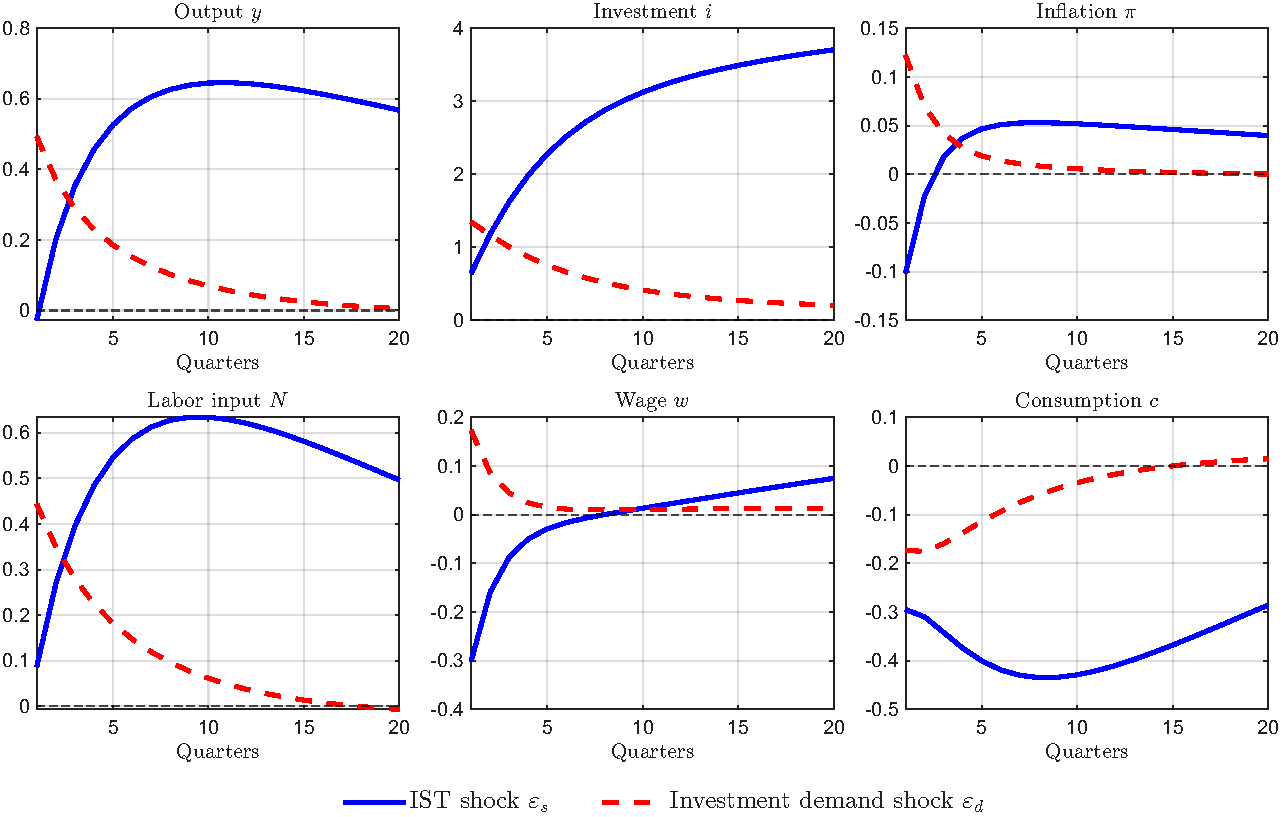
\includegraphics[width=\textwidth]{figures/compare_irf_gov_data.pdf}
\end{frame}

\begin{frame}{Historical decomposition (baseline)}
	\centering
	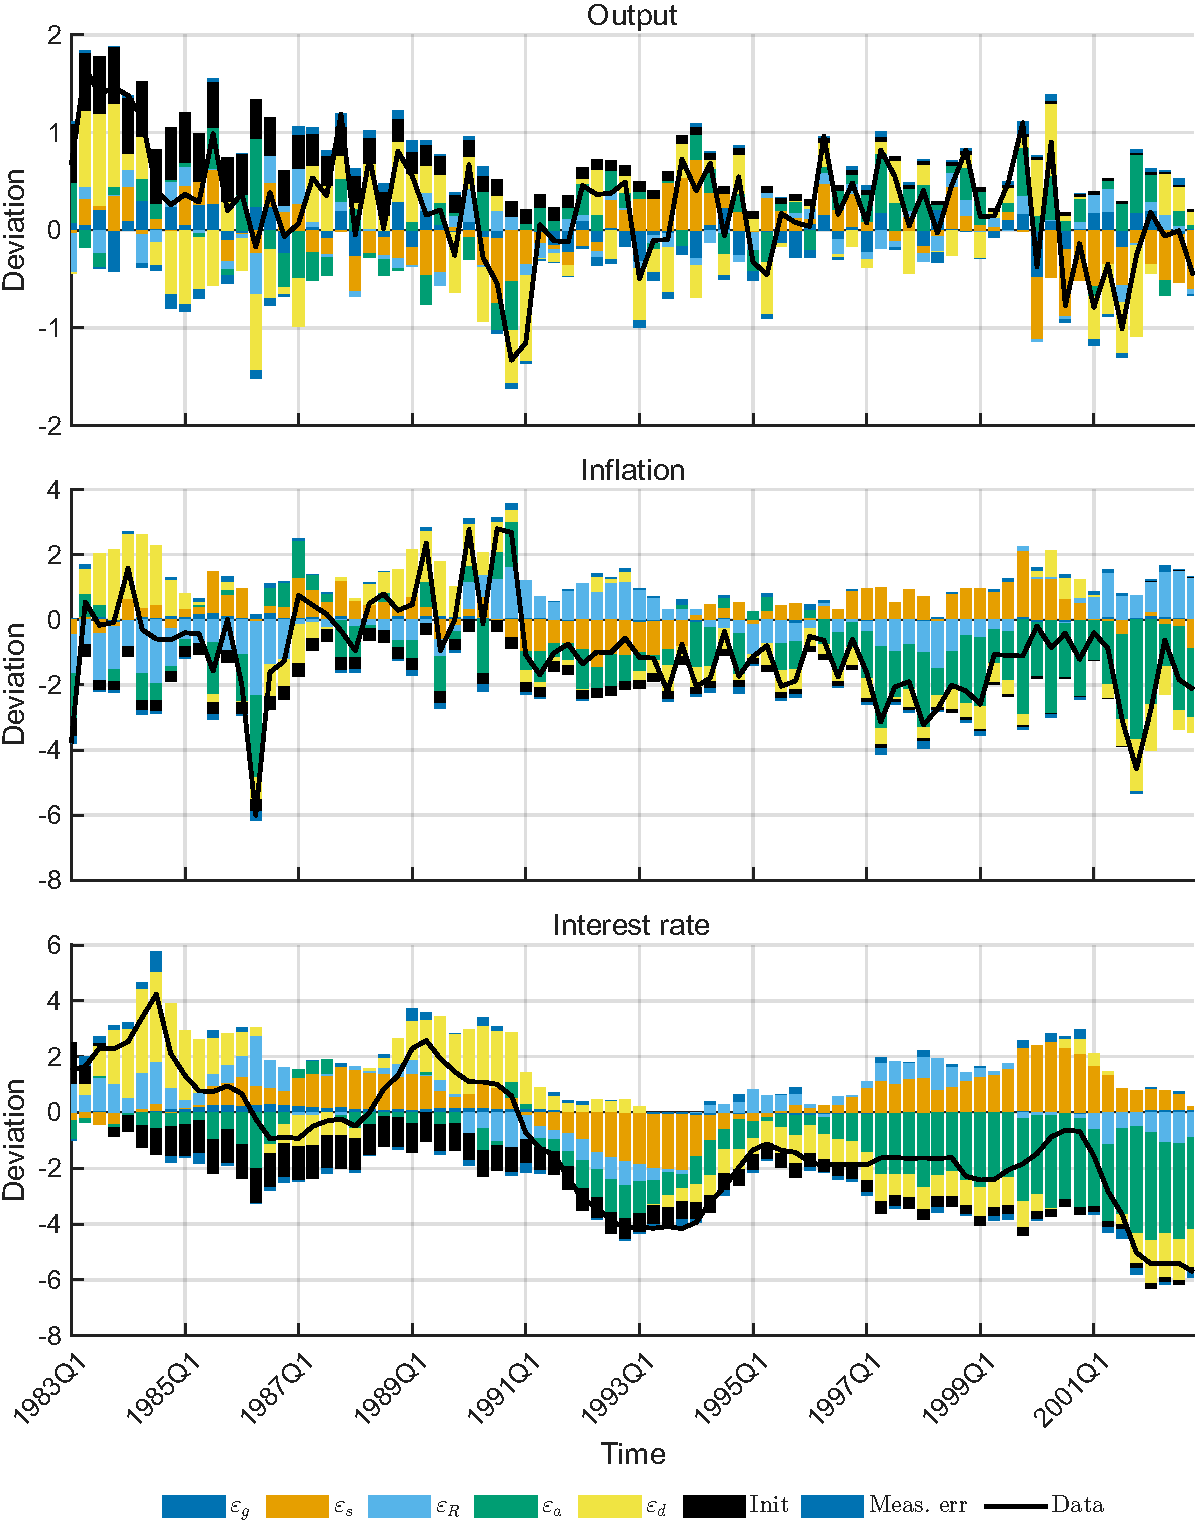
\includegraphics[width=0.6\textwidth]{figures/hd_gov_data.pdf}
\end{frame}

\begin{frame}{Robustness I: relative price disciplines IST}
	\begin{itemize}
		\item Add relative price of investment as an observable and interpret detrended relative price as inverse IST.
		\item Result: the inferred volatility/importance of IST falls; ID shock becomes more important in explaining macro fluctuations.
	\end{itemize}

	\vspace{0.4em}
	\centering
	{\scriptsize% Auto-generated by test_variance_decomp_nocap.m
% file_name: rel_price_data

\begin{table}[!htbp]
\centering
\caption{Unconditional FEVD (\%) for the model estimated with the relative price of investment as an additional observable, by structural shocks.}
\label{tab:vd:rel-price-data}
\begin{tabular}{l @{\hspace{2em}}r @{\hspace{2em}}r @{\hspace{2em}}r @{\hspace{2em}}r @{\hspace{2em}}r}
\hline\hline
Observable & $\varepsilon_g$ & $\varepsilon_{s}$ & $\varepsilon_R$ & $\varepsilon_a$ & $\varepsilon_{d}$ \\ 
\hline
Output & 5.72 & 0.59 & 17.21 & 17.86 & 58.61 \\ 
Inflation & 0.78 & 2.84 & 13.15 & 73.26 & 9.97 \\ 
Interest rate & 1.10 & 4.06 & 7.02 & 74.88 & 12.94 \\ 
Hours & 7.74 & 8.29 & 2.25 & 38.17 & 43.55 \\ 
Investment & 0.21 & 1.73 & 0.59 & 9.61 & 87.86 \\ 
Gov. spending & 99.44 & 0.00 & 0.10 & 0.11 & 0.35 \\ 
Relative price & 0.00 & 100.00 & 0.00 & 0.00 & 0.00 \\ 
\hline
\end{tabular}
\end{table}
}
\end{frame}

\begin{frame}{Robustness II: Smets--Wouters-style expansion}
	\begin{itemize}
		\item Add key SW mechanisms: habit formation, monopolistic labor market structure, and additional shocks (preference + markup shocks).
		\item Add extra observables: consumption and wage growth.
		\item ID remains quantitatively important: about \textbf{25\%} of output FEVD and \textbf{78\%} of investment.
	\end{itemize}

	\vspace{0.2em}
	\centering
    {\scriptsize\input{tables/variance_decomp_sw_type.tex}}
\end{frame}

\begin{frame}{Takeaways}
	\begin{itemize}
		\item Estimated evidence supports an investment-demand-side driver of fluctuations in addition to IST.
		\item Baseline: ID shock delivers sizable FEVD shares and an inflationary expansion (vs IST deflationary).
		\item Robustness checks (relative price + SW-type model) preserve the main conclusion.
	\end{itemize}
\end{frame}

\begin{frame}[allowframebreaks]{References}
	\bibliography{reference}
\end{frame}

\begin{frame}{If we drop investment adjustment cost}
    \begin{figure}
        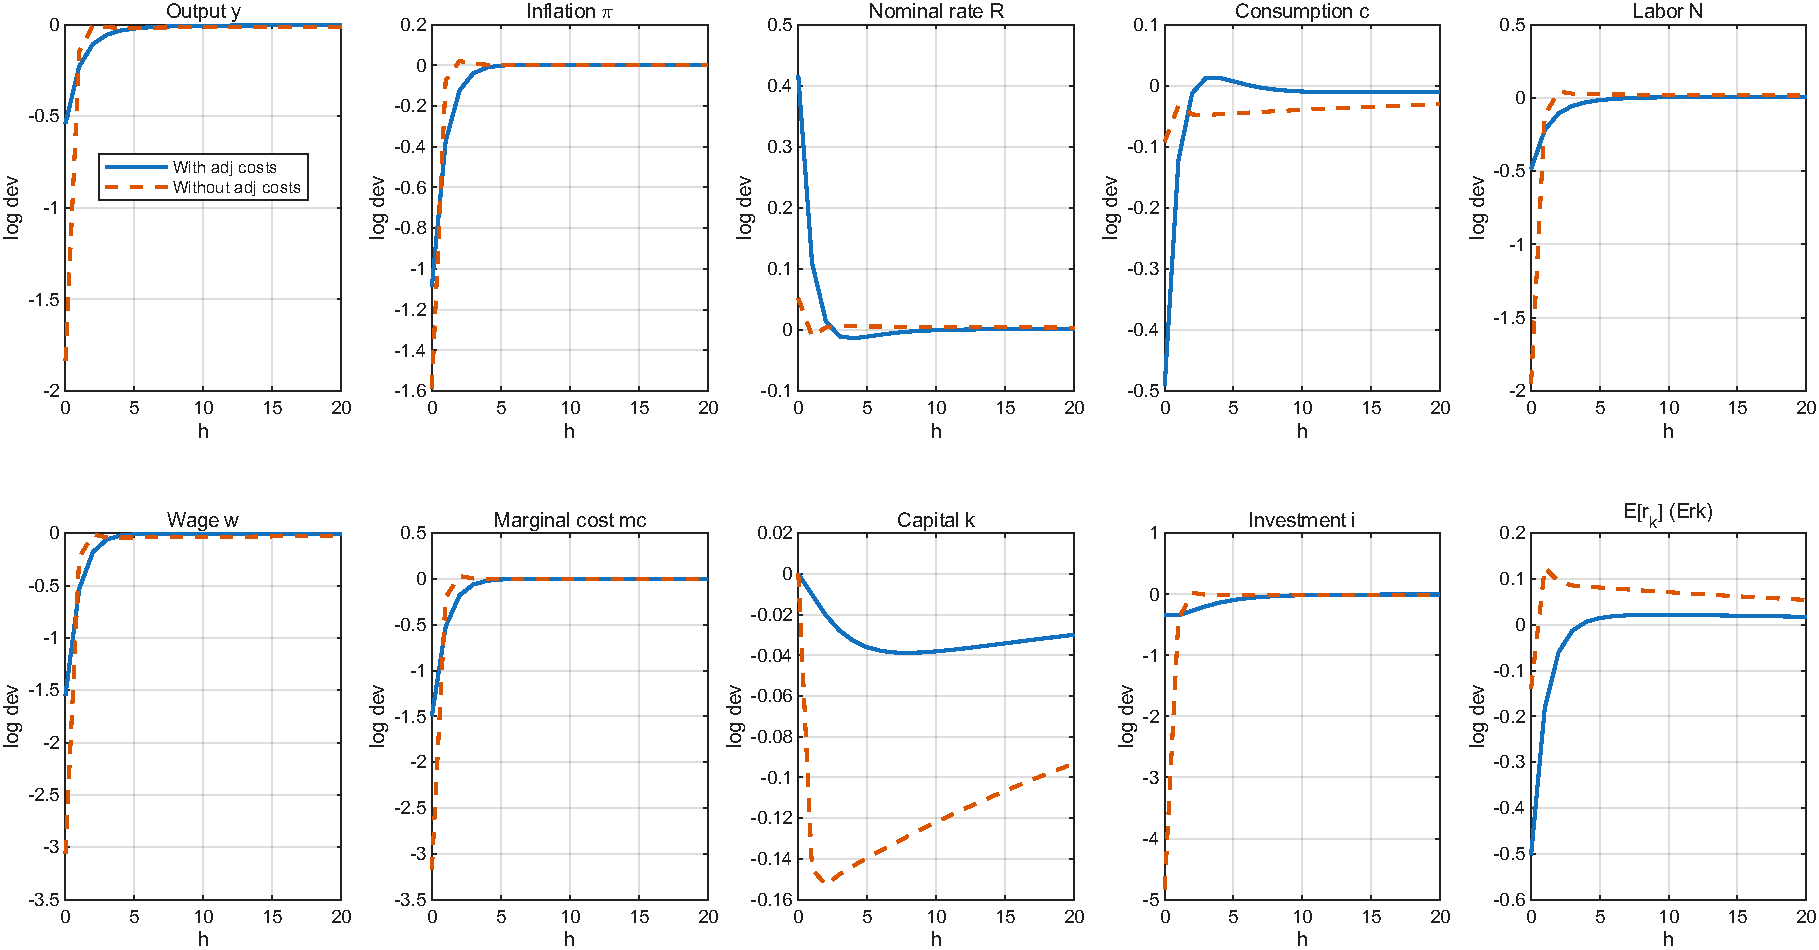
\includegraphics[width=\textwidth]{figures/CompareIRF_capital_utility_ratio.pdf}
        \caption{IRF: 1 s.d. monetary shock in the model with and without investment adjustment cost}
    \end{figure}
\end{frame}

\begin{frame}{If we don't use government spending data}
    % Auto-generated by test_variance_decomp_nocap.m
% file_name: invest_friction_without_z

\begin{table}[!htbp]
\centering
\caption{Unconditional Variance decomposition (\%).}
\label{tab:vd:invest-friction-without-z}
\begin{tabular}{l r r r r r}
\hline
Observable & $\varepsilon_g$ & $\varepsilon_{ist}$ & $\varepsilon_R$ & $\varepsilon_a$ & $\varepsilon_{id}$ \\ 
\hline
Output & 51.00 & 10.06 & 11.40 & 19.72 & 7.82 \\ 
Inflation & 15.19 & 37.49 & 16.06 & 30.65 & 0.61 \\ 
Interest rate & 20.64 & 47.73 & 5.36 & 25.92 & 0.35 \\ 
Hours & 85.73 & 11.27 & 0.43 & 2.25 & 0.32 \\ 
Investment & 0.24 & 61.13 & 0.90 & 14.32 & 23.40 \\ 
\hline
\end{tabular}
\end{table}

\end{frame}
\end{document}

